\documentclass[a4paper, 10pt]{article}
\usepackage[utf8]{inputenc}
\usepackage[english]{babel}
%\usepackage{etoolbox}
\usepackage[symbol]{footmisc}
%\usepackage{lmodern}
\usepackage[margin=2.5cm]{geometry}
\usepackage{hyperref}
\usepackage[section, boxed, prob-boxed, dem-boxed]{zeus}
\usepackage{mathtools}
\usepackage[only, mapsfrom]{stmaryrd}
\usepackage{parskip}
\setlist{nosep, noitemsep, label = (\textit{\roman*})}
\usepackage{todonotes}

\title{\sffamily \bfseries Algebraic Geometry\\Lecture Notes}
\author{\sc Guilherme Zeus Dantas e Moura\\\href{mailto:gdantasemo@haverford.edu}{\texttt{gdantasemo@haverford.edu}}}
\date{Haverford College\\Spring 2021\\ Last updated: \today}

\newcommand{\lecture}[3]{
	%\newpage
	%\section{#3 (#2)}
	\todo[bordercolor = gray!30!white, backgroundcolor = gray!30!white, noline]{\scalebox{.65}{\sf #2}}
}

\usepackage{import}
\usepackage{pdfpages}
\usepackage{transparent}
\usepackage{xcolor}

\newcommand{\incfig}[2][1]{%
    \def\svgwidth{#1\columnwidth}
    \import{./figures/}{#2.pdf_tex}
}

\newcommand{\correct}[2]{\textcolor{Red!90!black}{\st{#1}} \textcolor{ForestGreen}{#2}}
\newcommand{\signexpl}[3]{\underset{\substack{\uparrow\\\mathrlap{\text{\hspace{#3}#2}}}}{#1}}

\DeclareMathOperator\Aut{Aut}
\DeclareMathOperator\Hom{Hom}
\DeclareMathOperator\Tr{Tr}
\DeclareMathOperator\cod{cod}

\begin{document}
    \maketitle
	\sloppy
	
		This is Haverford College's undergraduate MATH H334, officially named Algebra II, instructed by Tarik Aougab.
		All errors are my responsability.

		Use these notes only as a guide. There is a non-trivial chance that some things here are wrong or incomplete (especially proofs).

		This class is being taught remotely via Zoom.
		
		\tableofcontents

	% start lectures
    \newpage
\lecture{1}{February 12, 2021}{Introduction}
\section{Introduction: It's all connected}

%\subsection{Markov Equation}
The Markov equation is \[
	x^2 + y^2 + z^2 = 3xyz.
\]

Let's understand the integer solutions for the Markov equation.

\begin{defn}[Markov number]
	A Markov number $n \in \NN$ is any number such that there exists $y_0, z_0$ such that $(n, y_0, z_0)$ is a solution to the Markov equation.
	Let $m_n$ be the $n$-th positive integer Markov number.
\end{defn}

\begin{exmp}[Markov number]
	$(1, 2, 5)$ is a solution to the Markov equation. Thus,  $1, 2, 5$ are Markov numbers.
\end{exmp}

%\subsection{Diophantine Approximation}

\begin{thm}[Caracterization of irrational numbers]
	Let $\alpha \in \RR$. Then, $\alpha$ is irrational $\iff$ there are infinitely many coprime $(p, q)$ such that \[
		\left|\alpha - \frac{p}{q}\right| < \frac{1}{\sqrt{5}q^2}.
	\]
\end{thm}

\begin{thm}[$\sqrt{5}$ is the best constant]
	If $\alpha = \phi = \frac{1 + \sqrt{5}}{2}$ and $\beta > \sqrt{5}$, there are only finitely many coprime  $(p, q)$ such that \[
		\left|\alpha - \frac{p}{q}\right| < \frac{1}{\beta q^2}.	
	\]
\end{thm}

If we disregard $\phi$ and its derivatives, then we can change $\sqrt{5}$ to $2\sqrt{2}$.

\begin{thm}[Caracterization of irrational numbers not related to $\phi$]
	Let $\alpha \in \RR$. Then, $\alpha \not\in \QQ[\phi]$ $\iff$ there are infinitely many coprime $(p, q)$ such that \[
		\left|\alpha - \frac{p}{q}\right| < \frac{1}{2\sqrt{2}q^2}.
	\]
\end{thm}

\begin{thm}[$2\sqrt{2}$ is the best constant]
	If $\alpha = \sqrt{2}$ and $\beta > 2\sqrt{2}$, there are only finitely many coprime  $(p, q)$ such that \[
		\left|\alpha - \frac{p}{q}\right| < \frac{1}{\beta q^2}.	
	\]
\end{thm}

We can disregard $\sqrt{2}$ and its derivatives, and change $2\sqrt{2}$ to $\frac{\sqrt{221}}{5}$; and so on.

This naturally creates a sequence of real numbers, called \emph{Lagrange numbers}, which starts as $\sqrt{5}$, $2\sqrt{2}$, $\frac{\sqrt{221}}{5}$, $\dots$, $L_n$, $\dots$.

%\subsection{Connection \# 1}

Surprisingly, there is a conection between the Markov and Lagrange numbers.

\begin{thm}[Markov]
	\[
		L_n = \sqrt{9 - \frac{4}{m_n^2}}
	\]
\end{thm}

%\subsection{}

\begin{thm}
	Let $\rho_1, \rho_2 \in \Hom(F_2, SL(2, \RR))$. If  $\Tr(\rho_1(a)) = \Tr(\rho_2(a))$, $\Tr(\rho_1(b)) = \Tr(\rho_2(b))$ and $\Tr(\rho_1(ab^{-1})) = \Tr(\rho_2(ab^{-1}))$, then there exists $A \in SL(2, \RR)$ such that $\rho_1(w) = A \rho_2 A^{-1}$ for all $w \in F_2$.
\end{thm}

The upshot of this theorem is that $\Hom(F_2, SL(2, \RR)) / \text{conjugation}$ is, in some sense, a subset inside $\RR^3$.

For certain homomorphisms $\rho: F_2 \to SL(2, \RR)$, there exists a magical machine, which we will call \emph{hyperbolic geometry machine}, that sends $\rho$ to the following figure.

\begin{figure}[ht]
    \centering
	\incfig[.5]{hyperbolic-geometry-machine-of-certain-homomorphisms}
    \caption{Result of the hyperbolic geometry machine on certain homomorphisms}
    \label{fig:hyperbolic-geometry-machine-of-certain-homomorphisms}
\end{figure}

The length of the blue, green and red loops are replated to $\Tr(\rho(a))$, $\Tr(\rho(b))$ and $\Tr(\rho(ab^{-1}))$.

For certain super special homomorphisms  $\rho: F_2 \to SL(2, \RR)$, this machine sends $\rho$ to this other figure.

\begin{figure}[ht]
    \centering
	\incfig[.5]{hyperbolic-geometry-machine-of-super-special-homomorphisms}
    \caption{Result of the hyperbolic geometry machine on super special homomorphisms}
    \label{fig:hyperbolic-geometry-machine-of-super-special-homomorphisms}
\end{figure}

\begin{thm}
	$\rho$ is super special if, and only if, \[\Tr(\rho(a))^2 + \Tr(\rho(b))^2 + \Tr(\rho(ab^{-1}) = \Tr(\rho(a))\Tr(\rho(b))\Tr(\rho(ab^{-1})),\] i.e., $\left(\frac{\Tr(\rho(a))}{3}, \frac{\Tr(\rho(b))}{3}, \frac{\Tr(\rho(ab^{-1}))}{3}\right)$ is a solution to the Markov equation.
\end{thm}

    \newpage
\section{Introducing Algebraic Varieties}
\lecture{2}{February 15, 2021}{Varieties in RR}

\subsection{Definition}

\begin{defn}[Affine hypersurface]
	Let $K$ be a field. $K[x_1, \dots, x_n]$ is the ring of polynomials with coefficients in $K$, and 

	Suppose $p \in K[x_1, \dots x_n]$ and $p$ is not constant. Then, \[
		V(p) := \left\{(k_1, \dots, k_n) \in K^n \mid p(k_1, \dots, k_n) = 0 \right\}
	\] 
\end{defn}

\begin{exmp}
	Let $K = \RR$ and $n = 2$. Consider $p(x_1, x_2) = x_1^2 + x_2^2 - 1$. In this case, \[
		V(p) = \{(r_1, r_2) \in \mathbb{R}^2 \mid r_1^2 + r_2^2 - 1 = 0\}.
	\]

	In this case, $V(p)$ represents a circle.

	More generally, ellipses, hyperbolas, parabolas are all $V(p)$, for the right choice of $p$.
\end{exmp}

\begin{defn}[Algebraic variety]
	More generally, if $\mathcal{P}$ is a collection of polynomials in $K[X]$, not constants. Define \[
		V(\mathcal{P}) = \{(k_1, \dots, k_n) \in K^n \mid p(k_1, \dots, k_n) = 0, \forall p \in \mathcal{P}\}.
	\] 
\end{defn}

\subsection[Examples in real numbers]{Examples with $K = \RR$}

\begin{ques}
	What sorts of geometric properties can algebraic varieties have?
\end{ques}

\begin{exmp}
	Consider $p(x, y) = y^2 - x^3$.  Then, $V(p)$ looks like:
	\begin{center}
		
\includegraphics[width = .25\textwidth]{figures/variety_example_1.pdf}
	\end{center}
\end{exmp}

\begin{exmp}
	Consider $q(x, y) = y^2 - x(x^2 - 1)$. Then,  $V(q)$ looks like:
	\begin{center}
		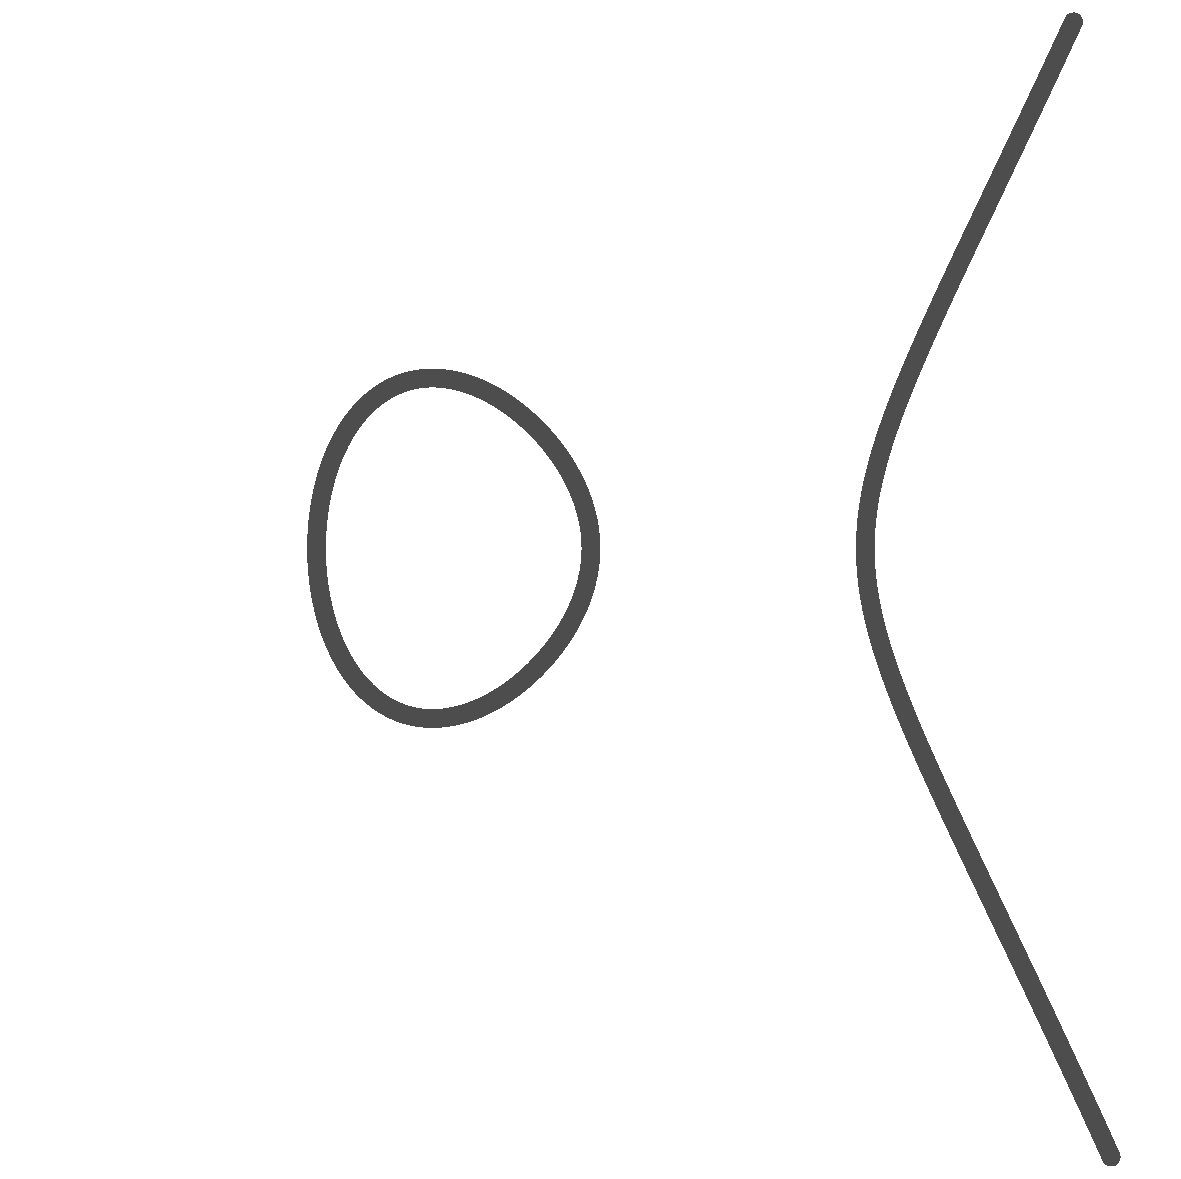
\includegraphics[width = .25\textwidth]{figures/variety_example_2.pdf}
	\end{center}
\end{exmp}

\begin{exmp}
	Consider $r(x, y) = y^2 - x^2(x+1)$. Then, $V(r)$ looks like:
	\begin{center}
		
\includegraphics[width = .25\textwidth]{figures/variety_example_3.pdf}
	\end{center}
\end{exmp}

\begin{exmp}
	Consider $s(x, y) = xy$. Then, $V(s)$ looks like:
	\begin{center}
		
\includegraphics[width = .25\textwidth]{figures/variety_example_4.pdf}
	\end{center}
\end{exmp}

\begin{defn}
	We say a variety has dimension $d$ if a subset of it ``looks like $\mathbb{R}^d$'' and if it is the disjoint union of finitely many pieces that each ``look like  $\mathbb{R}^i$'' with $0 \le i \le d$
\end{defn}

\begin{exmp}
	The dimension of $V(x^2 + y^2 - 1)$ is $1$.
\end{exmp}

\begin{exmp}
	The dimension of $V(\{x, y\}) = \{(0, 0)\}$ is $0$.
\end{exmp}

In Linear Algebra, the number of linearly independent always equals the codimension of the solution set.

\begin{ques}
	Does this hold for varieties?
\end{ques}
\begin{ans}
	No. $V(x^2 + y^2) = \{(0, 0)\}$, which has dimension $0$ (as opposed to the expected $2 - 1 = 1$). Another example is $V(y, y - 1) = \varnothing$, which has dimension $-1$ (as opposed to the expected $2 - 2 - 2$).
\end{ans}

So, linear algebraic dimension count fail for varieties for at least two reasons:
\begin{enumerate}[label = \textbullet]
	\item non-existence of solutions to certain types of algebraic equations (e.g., $x^2 = - 1$).
	\item non-extistence of intersections between parallel lines.
\end{enumerate}

    \lecture{3}{February 17, 2021}{\PP(\CC)}

To solve the first problem, we'll use the complex numbers instead of the real numbers. To solve the second problem, we'll need to develop \emph{projective spaces}.

\newpage
\section{Introducing Projective Spaces}

\paragraph{Basic idea} Start with a initial space and add new point to it which keep track of the different ``ways'' of goign off to infinity in a straight line. 

\paragraph{Notation} $\PP^{\text{dimension}}(\text{field})$.

\begin{exmp}[Real projective line]
	Consider the projective space $\PP^1(\RR)$: this is just $\RR$ plus one additional point ``at infinity''.
\end{exmp}

\begin{exmp}[Real projective plane]
	Consider the projective space $\PP^2(\RR)$: this is  $\RR^2$ plus an additional point for each line in  $\RR^2$ through the origin.

	Any two parallel lines in $\RR^2$ intersect in the $\PP^2(\RR)$.

	So, any two lines in $\PP^2(\RR)$ intersect at a point in  $\PP^2(\RR)$
\end{exmp}

\begin{exmp}[Complex projective line]
	Consider the projective space $\PP(\CC)$: this is just $\CC$ plus one additional point ``at infinity''.
\end{exmp}

%\begin{defn}
%	In $\CC^2$, a \emph{complex line through the origin} is a subset of $\CC^2$, say $A$, satisfying that for all $\lambda \in \CC$ such that  \[
%		(z, w) \in A \iff (\lambda z, \lambda w) \in A.
%	\]
%
%	(This definition allows $A = \varnothing$, $A = \{0\}$ and $A = \CC^2$, but we will disregard those.)
%\end{defn}

\begin{defn}
	In $\CC^2$, a \emph{complex line through the origin} is a subvector space of $\CC^2$ over $\CC$ with dimension $1$.
\end{defn}

    \lecture{4}{February 19, 2021}{}

\begin{exmp}
	Consider the projective space $\PP^2(\CC)$: this is  $\CC^2$ plus an additional point ``at infinity'' for each complex line through the origin.

	``How many'' new points are there? There is one for each complex line. In fact, if we look to the ``slope'' of each complex line, it lives inside $\PP(\CC)$ and uniquely identifies each complex line.
\end{exmp}


    \newpage
\section{Exploring some varieties}
\lecture{5}{February 26, 2021}{Starting to do real math}

\begin{exmp}
	\[
		y^2 = ...
	\]
	yields a sphere on $\PP^2(\CC)$.
\end{exmp}

\begin{exmp}
	\[
		y^2 = x(x^2 - 1)
	\]
	yields a torus on $\PP^2(\CC)$.
\end{exmp}

\begin{thm}[WRONG! Dream Theorem]

\end{thm}

\begin{exmp}
	The polynomial $p(x, y) = xy$ yeilds to two spheres that touch at one point in $\PP^(\CC^2)$; which is not on the list.
\end{exmp}

\begin{thm}[Correct Theorem]
	If $p \in \CC[x, y]$ ...
\end{thm}

    \newpage
\section{Projective Spaces}
\lecture{6}{March 01, 2021}{Let's start do definitions}

Let $K$ be a field (in practice, for this class, $K = \RR$ or $\CC$).

\begin{thm}[$n$-dimension Projective Space]
	Given $n \in \ZZ_{\ge 0}$, the projective $n$-dimension space over $K$, denoted by $\PP^n(K)$, is defined as the set \[
		\PP^n(K) = \{A \subset K^{n+1} : A \text{ is a subspace of } K^{n+1} \text{ with dimension }1 \text{over $K$} \}	
	\]
\end{thm}

\paragraph{Small, informal aside:} $\PP^n(K)$ is more than just a set. It is a topological space --- more on this soon.

\begin{exmp}
	$\PP^1(\RR)$ is the set of lines in $\RR^2$ that go through the origin.

	We can try to use the blue circle to ``keep track'' of the lines.
\end{exmp}

\begin{figure}[ht]
    \centering
    \incfig{projective-real-line}
    \caption{Projective real line}
    \label{fig:projective-real-line}
\end{figure}

\begin{exmp}
	$\PP^2(\RR)$ is the set of lines in $\RR^3$ that go through the origin. 

	We can try to use the unit sphere to ``keep track'' of the lines.
\end{exmp}

\begin{defn}
	If $U$ is a $(r+1)$-dimensional subspace of $K^{n+1}$, then the $1$-subspaces of $U$ yield a subset of $\PP^n(K)$, and called a $r$-dimension projective subspace.
\end{defn}

\begin{prop}
	Any $r$-dimension projective subspace is naturally a copy of $\PP^r(K)$ inside of $\PP^n(k)$.
\end{prop}
\begin{dem}
	Any two $r$-dimension subspaces of $K^{n+1}$ are related by an isomorphism of  $K^{n+1} \to K^{n+1}$ (change of basis). Notice also that  $K^{r+1} \subset K^{n+1}$, corr. to zero-ing out the last  $n-r$ coordinates is an $(r+1)$-subspace of $K^{n+1}$. And its $1$-subspaces are the elements of $\PP^r(K)$, by definition.
\end{dem}

\begin{defn}
	If a vector space $V$ has dimension $n$, and $U \subset V$ is a subspace, the \emph{co-dimension of $U$}, denoted $\cod(U)$, is  \[
		\cod(U) = n - \dim(U).
	\]
\end{defn}

\begin{lem}
	Let $S_1, S_2$ be any two projective subspaces of $\PP^n(K)$. Then, \[
		\cod(S_1 \cap S_2) \le \cod(S_1) + \cod(S_2).
	\]

	Equivalentely, \[
		\dim(S_1 \cap S_2) \ge \dim(S_1) + \dim(S_2) - n.
	\]
\end{lem}

    \lecture{7}{March 03, 2021}{}

\begin{sk}
	Using tools from Linear Algebra, we can conclude that given two subspaces $V_1, V_2 \subset V$, \[
		\dim(V_1 \cap V_2) \ge \dim(V_1) + \dim(V_2) - \dim(V). 
	\]

	An $(r+1)$-dimensional subspace $\tilde S_1$ of $K^{n+1}$ has codimension $(n+1) - (r+1) = n - r$. And, the associated projective subspace $S_1$ of $\PP^n(K)$ has same codimension. So, the inequality for vector spaces implies the inequality for projective spaces.
\end{sk}

We will use a lot the connection between vector spaces and projective spaces.

\begin{exmp}
	Any two projective $2$-spaces in $\PP^3(\RR)$ intersect in at least a (projective) line.
\end{exmp}

\begin{defn}
	Let $p \in \PP^n(K)$ --- we may call $p$ a \emph{projective point}, or simply a \emph{point} --- and let $L_p$ be the corresponding line throught the origin in $K^{n+1}$. (\emph{Technically, those are the same, but it is useful to separate them.})

	Then, if $\vec a \in K^{n+1}$, $\vec a \in L_p$, $\vec a \neq \vec 0$, we call  $\vec a$ a \emph{coordinate set for $p$} --- or simply \emph{coordinates for $p$}.
\end{defn}

An unforunate fact is that a single projective point $p$ doesn't have a unique coordinate set.

\begin{prop}
	Given two non-zero $\vec a, \vec b \in K^{n+1}$, they are coordinate for the same point in $\PP^n(K)$ if, and only if, there exists $\lambda \in K$ such that \[
		\vec a = \lambda \cdot \vec b,
	\]
	i.e., if $0$, $\vec a$ and $\vec b$ are collinear.
\end{prop}

\begin{exmp}
	Let's think about $\PP^2(\RR)$.

	For any point $(x, y, z) \in \RR^3$ such that $z \neq 0$, we can divide by $z$ and get $\left(\frac{x}{z}, \frac{y}{z}, 1\right)$ --- \emph{which represents the same projective point in $\PP^2(\RR)$ as $(x, y, z)$.}

	Therefore, except for the projective points (lines) in the $xy$-plane, we can handle the problem of non-unique representation of projective points by referring to a projective point by the \emph{unique} point in $\RR^3$ with a $1$ in the last coordinate. See \cref{fig:real-projective-plane}.

	So, the plane $z = 1$ (a copy of $\RR^2$) can be naturally identified with the subset of $\PP^2(\RR)$ consisting of projective points that represent lines \emph{not} in the $xy$-plane.
	The remaining projective points can be identified with a copy of $\PP^1(\RR)$ --- which we usually call \emph{the line at infinity}.

	In general, one can always imagine $\PP^n(K)$ as a copy of $K^n$ together with a copy of $\PP^{n-1}(K)$ \emph{``at infinity''} --- the latter we call \emph{the hyperplane at infinity}.
\end{exmp}

\begin{rem}
	There is no preferred hyperplane at infinity. In our example, the choice of the plane $z = 1$ was completely arbitrary.
\end{rem}

\begin{figure}[ht]
    \centering
	\incfig[.6]{real-projective-plane}
    \caption{Real Projective Plane}
    \label{fig:real-projective-plane}
\end{figure}

\begin{lem}
	Any $(n-1)$-dimensional projective subspace $W$ in $\PP^n(K)$ can be chosen as the hyperplane at infinity.
\end{lem}

	% end lectures
\end{document}
